\documentclass{article} % For LaTeX2e
\usepackage{nips14submit_e,times}
\usepackage{graphicx}
\usepackage{hyperref}
\usepackage{caption}
\usepackage{subcaption}
\usepackage{url}
%\documentstyle[nips14submit_09,times,art10]{article} % For LaTeX 2.09
\usepackage{array} 


\usepackage{amsmath, amsthm, amssymb, amsfonts}
\usepackage{bm}
% Macro definitions for mathy stuff
\DeclareMathOperator{\identity}{\mathbb{I}}
\DeclareMathOperator{\E}{\mathbb{E}}
\DeclareMathOperator{\BigO}{\mathcal{O}}
\newcommand{\norm}[1]{\left\lVert#1\right\rVert}
\newcommand{\infnorm}[1]{\norm{#1}_{\infty}}
\newcommand*\mean[1]{\overline{#1}}
\newcommand*{\expect}[1]{\E\left[ #1\right]} % expectation value
\newcommand*{\expectover}[2]{\E_{#1} \left[ #2 \right]} % expectation value w/subscript
\newcommand{\refeq}[1]{\mbox{eq.(\ref{#1})}}
\newcommand{\vect}[1]{\mathbf{#1}}
\newcommand{\mat}[1]{\mathbf{#1}}

\title{Predicting gender from OKCupid profiles using ensemble methods}


\author{Isaac Backus}

\newcommand{\fix}{\marginpar{FIX}}
\newcommand{\new}{\marginpar{NEW}}

\begin{document}


\maketitle

\begin{abstract}
In this paper I explore a method for predicting the sex of OKCupid users.  Only male/female are options in this dataset.  Missing data is replaced through mean imputation, although other methods are tried.  8 models (7 coded by me, 1 from scikit-learn) are trained on the data.  Their results are combined with the ensemble method of stacking which uses a weighted sum of the models' predictions.  This method is able to predict the sex of users with an 89\% success rate.
\end{abstract}

\section{Introduction}
\label{sec:introduction}
Ensemble methods in machine learning can present a simple but powerful method of combining the predictions of several, or many, machine learning algorithms into an ensemble model which is a better predictor than every individual model used.

In this paper I explore using the ensemble method of stacking, which combines predictions through a weighted sum, to predict the sex of people on OKCupid from a limited set of profile questions\footnote{In my original proposal I was going to predict incomes, but I realized that the response rate to incomes was very low (1/6) and from linear regression it appeared there were many outliers who may have been misreporting their income.  This leaves too small of a usable dataset.  For this reason I switched to predicting sex.}.  All the machine learning code was written by me, except one model (a random forest from scikit-learn) which I used primarily to verify my methods.  In \S\ref{sec:features} I outline the dataset and the methods I used for generating features from it.  In \S\ref{sec:missing_data} I explain how I handled missing data, since this dataset is a questionnaire with an 87\% response rate to questions.  In \S\ref{sec:models} I outline the 8 models trained and explain the ensemble method to combine their predictions in \S\ref{sec:ensemble}.  Results are presented in \S\ref{sec:results} and discussed, along with possible improvements to my methods, in \S\ref{sec:discussion}.  I find that I am able to predict sex (from one of male or female) with an 89\% success rate.

\section{Generating Features}
\label{sec:features}
The dataset is a text .csv document available on GitHub\footnote{\url{https://github.com/rudeboybert/JSE_OkCupid.git}}, made freely available by OKCupid.  The entries are responses to a 31 questions by 59946 people within 25 miles of San Francisco with at least one profile picture who were online during 2011-2012, all of whom were over 18 (at least according to their profiles).  The respondents in this dataset are 40.2\% female (class 0) and 59.8\% male (class 1).  The ages have a range of 18-69 with a mean of 32.3 and a standard deviation of 9.4.  This is sample is clearly not representative of the population at large.

Generating usable features for this dataset required parsing.  Two methods were used which generated 217 and 101 features.  I explain those methods here.  After features were generated, the data set was split up into training and test sets of 49946 and 10000 entries, respectively, by randomly choice.

\subsection{Full feature set}
\label{sec:full_features}
10 of the profile questions were short responses to prompts such as \textit{What I'm doing with my life} or \textit{On a typical Friday night I am...}.  Since natural language processing was outside of the scope of this project, these were discarded.  The remaining 21 responses were numbers, binary choices, multiple choice, multiple choice-multiple response, or ranked multiple choice responses and were all handled differently.

Numbers, such as height, age, or income, were left unaltered.  Binary choices such as \textit{sex} were converted to 0/1 according to the (alphabetized) options.  So female (male) go to 0 (1).  Multiple choice responses such as \textit{pets} were converted multiple binary features (one for each choice).  A response to \textit{pets} of \textit{has dogs and likes cats} would be converted (under the assumption that dog owners like dogs) to: (\textit{has dogs, likes dogs, has cats, likes cats}) = (1, 1, 0, 1).
%\begin{center}
%	\begin{tabular}{cccc}
%		has dogs & likes dogs & has cats & likes cats \\ 
%		1 & 1 & 0 & 1
%	\end{tabular}
%\end{center}

Certain questions, such as languages spoken, allowed multiple responses to be given, with possible modifiers.  Someone who speaks English fluently and Chinese alright might respond \textit{English (fluently), Chinese (okay)}.  Speaking a given language poorly was counted as not speaking it, otherwise you are counted as a speaker.  A binary feature was then made for each language, marking a 1 for each language a person speaks.  This generates many (76) features which is addressed  in \S\ref{sec:pared_features}.  The two ranked multiple-choice questions were about drugs and drinking.  These were assigned numbers 0, 1, 2, ... indicating the amount of use.

Features with a response rate lower than 25\% were dropped (including income).  Finally, the data was conditioned by subtracting the mean of each feature and normalizing by the standard deviation of each feature.  This procedure generated 217 features which I call the full feature set.

\subsection{Pared feature set}
\label{sec:pared_features}

Certain questions created many features (because of their many possible responses), which all had very small regression weights (see \S\ref{sec:models}).  To see if this is an issue, I created a pared down feature set.  I reduced the number of language of features  from 76, one for each language), to 3: (i) a binary choice for speaking English; (ii) the number of languages a person speaks; (iii) and I retained \textit{speaks\_c++} since that was a good predictor of sex (being male).

I retained responses to how much astrological sign matters (\textit{it doesn't matter}, \textit{it matters a lot}, or \textit{it's fun to think about}) and recorded whether or not the person reported their sign and discarded the astrological sign features. Education was also a multiple choice question with many possible responses, such as \textit{high school} or \textit{dropped out of college}.  I created a ranking by hand of education with numbers of 1-28 with 1 being \textit{dropped out of high school} and 28 being \textit{graduated from ph.d program} and replaced the education features by a single feature.

As with the full set, the data was conditioned by subtracting the mean of each feature and normalizing by the standard deviation of each feature.  This created a set of 101 features.

\section{Missing Data}
\label{sec:missing_data}
Around 13\% of these features had no response.  Restricting the dataset to only people/questions will full responses would have narrowed the dataset to a tiny fraction of its initial size and may have biased the data.  Therefore, 3 imputation methods were tested.

The simplest technique---which was ultimately used---was mean value imputation.  Missing entries were replaced with their feature means.  This technique underestimates feature variances and does ignore any possible correlations between among features and ignores the possible importance of choosing to not answer a question.  I also tested random selection, whereby missing entries are replaced by randomly chosen entries (from the same feature).  This was as successful as mean value imputation under logistic regression.

I also tried using regression models for missing data imputation, but this failed with my dataset.  First, missing values were replaced by mean value imputation.  A feature was then selected and treated as training labels. A linear model was trained on the data with responses, which could be used to predict missing values (see~\S\ref{model:linear}).  This was repeated for all features and the missing values were replaced by their predictions.  Examining the predictions of the models showed many poorly predicted features (see Figure~\ref{fig:linear_imputation}).  This method was therefore dropped in favor of mean value imputation.

\begin{figure}[]
\centering
\begin{subfigure}{0.5\textwidth}
	\centering
	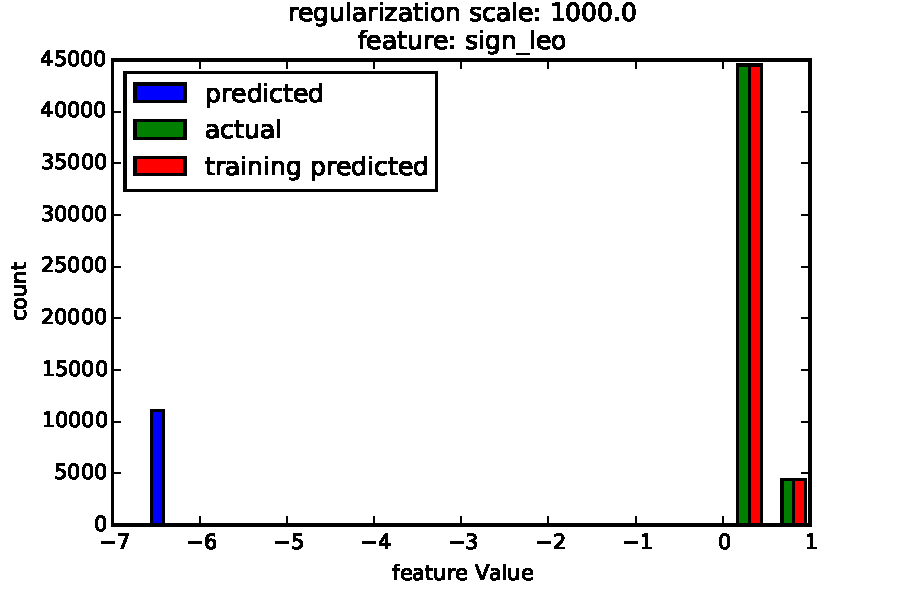
\includegraphics[width=0.9\linewidth]{figures/imputed_dist_sign_leo.pdf}
	\caption{}
	\label{fig:imputed_dist_sign_leo}
\end{subfigure}%
\begin{subfigure}{0.5\textwidth}
	\centering
	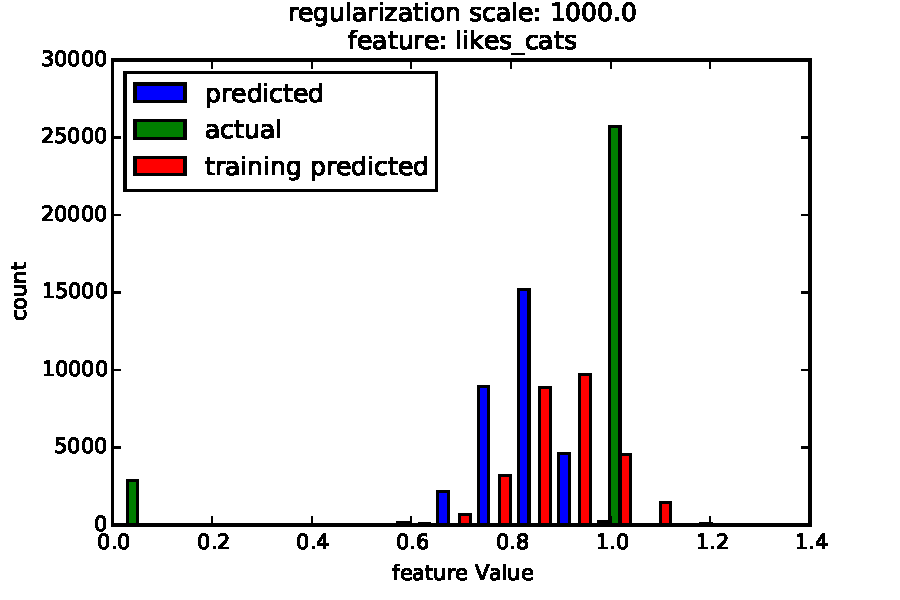
\includegraphics[width=0.9\linewidth]{figures/imputed_dist_likes_cats.pdf}
	\caption{}
	\label{fig:imputed_dist_likes_cats}
\end{subfigure}%
\caption{Regression imputation.  Histograms of predictions from linear regression for features compared to actual values.  Under the regression imputation, these models would be used to predict missing values.  For features which are uncorrelated with the rest of the data and have mainly one response, such as astrological signs (\ref{fig:imputed_dist_sign_leo}), predictions can be wildly off.  Other features fair better and capture the mean well but don't separate the data into multiple populations well and are not very good predictors (\ref{fig:imputed_dist_likes_cats}).
}
\label{fig:linear_imputation}
\end{figure}


\section{Models}
\label{sec:models}
A total of 8 different models were trained on the data.  7 of these were written by me in python using numpy and scipy.  Additionally, a random forest model was trained using scikit-learn, which was chosen primarily as a verification that my methods were indeed working and were performing well given the data.  Results for these models are presented in table~\ref{table:results}.  These models were then combined using an ensemble method, detailed in \S\ref{sec:ensemble}.  

Here I explain the models used and present their results.

\subsection{Linear (ridge) regression}
\label{model:linear}
A standard ridge regression was very useful to implement, since implementation is fast and training/prediction are very quick.  Under ridge regression, y values are predicted according to a linear model:
\begin{align}
\label{eq:linearmodel}
\vect{\hat{y}} &= \mat{X}\vect{\hat{w}} + \hat{w_0} \\
\label{eq:ridge_weights}
\vect{\hat{w}} &= \left( \mat{X^T} \mat{X} + \lambda \identity  \right)^{-1} \mat{X}^T \vect{y}
\end{align}
Where $\mat{X}$ is the training data and $\vect{y}$ is the training labels. The regularization I used here was $\lambda = 10./mean(\mat{X}^2)$ where the square is element-wise, chosen by selecting the largest value which gave a good squared training loss.

Classification is performed by classifying data points with $\vect{\hat{y}}$ bigger than some threshold as class 1 and the others as class 0.  The threshold was found by choosing a threshold that minimizes the 0/1 loss on the training set by considering many threshold values within the range of $\vect{\hat{y}}$. 

For the ensemble method (\S\ref{sec:ensemble}) it is good to have some way of quantifying the confidence (or the probability) of these predictions.  This is not inherent to a linear model such as this, so I used a simple heuristic.  The confidence of being in class 1 is given by:
\begin{equation}
C_0(y) = \frac{n_{0>}}{n_{1<} + n_{0>}}
\end{equation}
where $n_{0>}$ is the number of training points of class 0 greater than $y$ and $n_{1<}$ is the number of training points in class 1 less the $y$.  The confidence of being in class 0 is $1-C_0$.  This gives a confidence of 1 in regions at the extremes of $\vect{\hat{y}}$ where all training points are in one class or the other.  The confidences are then rescaled to $C_1$ such that at the threshold $C_1=0$.  This method seems to over-predict the confidences, with a strong emphasis on $C_1 = 1$, but it is still better than just a binary prediction for the ensemble method used below.

%\begin{figure}[]
%	\centering
%	\begin{subfigure}{0.45\textwidth}
%		\centering
%		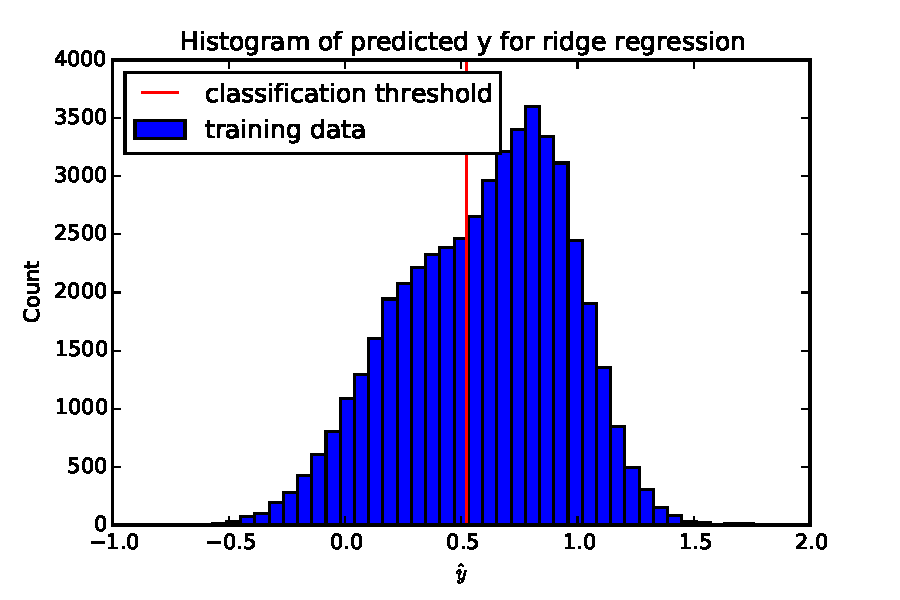
\includegraphics[width=0.9\linewidth]{figures/linear_ypred_histogram.pdf}
%		\caption{Histogram of $\vect{\hat{y}}$ for the training set for the ridge regression.  Values larger than the threshold are classified as class 1 (male), values less than the threshold are classified as 0 (female).}
%		\label{fig:ridge_ypred_hist}
%	\end{subfigure}%
%	\hfill
%	\begin{subfigure}{0.45\textwidth}
%		\centering
%		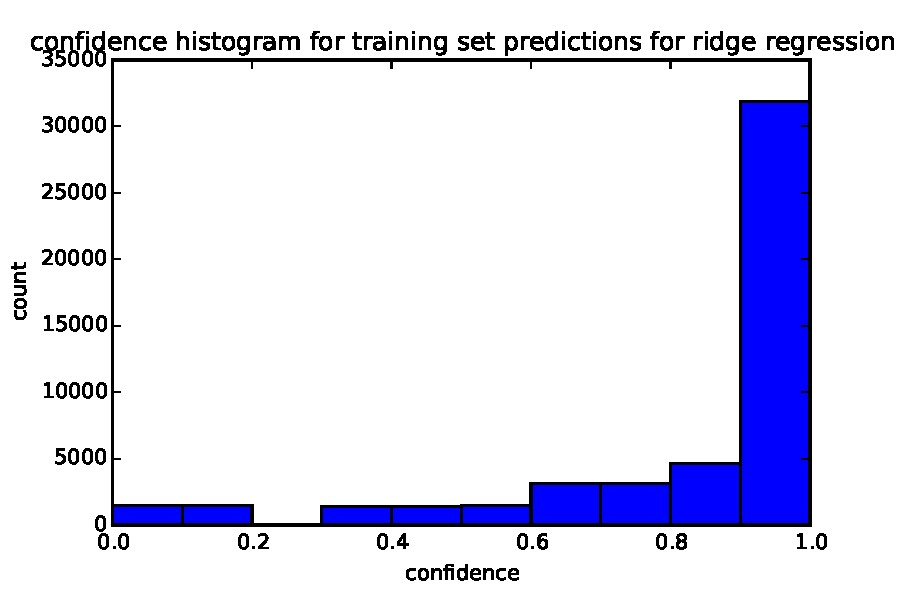
\includegraphics[width=0.9\linewidth]{figures/ridge_confidence.pdf}
%		\caption{Histogram of prediction confidences for the ridge regression.  Confidences may be overestimated.}
%		\label{fig:ridge_confidence_hist}
%	\end{subfigure}%
%	\caption{Results of the ridge regression of \S\ref{model:linear}.}
%	\label{fig:ridge_histograms}
%\end{figure}

\subsection{Logistic regression}
\label{model:logistic}
The logistic model predicts the probability that a data point $\vect{x}$ belongs to class 1 according to:
\begin{equation}
\label{eq:logistic}
p(\vect{y_i}=1 | \vect{x_i}) = \frac{1}{1 + \exp[-(\vect{x_i}\cdot\vect{w} + w_0)]}
\end{equation}
The weights $\vect{w}, w_0$ were trained using a stochastic gradient descent (SGD) algorithm that I wrote.  In my algorithm, the data is randomly shuffled after each epoch and weight updates are performed in mini-batches.  As in any SGD, the weights were updated by calculating the gradient of the loss function:
\begin{align}
\label{eq:sgd_weight_update}
\vect{w'} &= \vect{w} - \eta \nabla_{\vect{w}} L \\
\label{eq:logistic_loss}
L &= \lambda \norm{\vect{w}}^2 -\frac{1}{N}\sum_{i=1}^{N} \ln(p_i)
\end{align}
where $\eta$ is the learning rate (a parameter). The gradient of the loss is can be calculated analytically from this and eq.\ref{eq:logistic}.
Since the SGD is effectively regularized, I used $\lambda=0$.  I used a mini-batch size of 100.  I set the convergence criterion to be when the log-loss had a fractional decrease of less than $10^{-6}$.  A powerlaw learning rate was used according to:
\begin{equation}
\label{eq:learning_rate}
\eta = \frac{\eta_0}{(1 + k/\tau)^\kappa}
\end{equation}
where$k$ is the total number of data points that have traversed.  For the logistic regression I used $\eta_0 = 0.1/mean(\mat{X}^2)$, $\tau = 10^5$, and $\kappa = 0.55$.  The algorithm converged after 14 epochs.

\subsection{L2 Boosted Ridge Regression}
\label{model:l2boost}
Since the ridge regression ended up being as good as the best algorithms (see~\S\ref{sec:results}), I decided to attempt a boosted ridge regression.  The algorithm for this L2 boosted ridge regression is as follows.
\begin{enumerate}
	\itemsep-0.2em 
	\item Initialize a while loop by setting a predictor $f^{(0)}(\mat{X}) = 1 $ and setting $m=0$.
	\item Train a linear model $g^{(m)}(\mat{X}) = \mat{X}\vect{w^{(m)}} + w_0^{(m)}$ via ridge regression on the residuals vector $\vect{U} = f^{(m)}(\mat{X}) - \vect{y}$. 
	\item Update the model by setting $f^{(m+1)}(\mat{X}) = f^{(m)}(\mat{X}) + \nu g^{(m)}(\mat{X})$ where $\nu \in (0, 1]$ is a tuneable parameter (I chose 0.5).  Then increment $m$ and loop over steps 2-3 until the maximum number of iterations is reached
\end{enumerate}
I stopped iterating when the 0/1 loss on the training set of $f^{(m)}$ converged (10 iterations).  This is a linear model which weights misclassified points more heavily by fitting the residuals.  Classification and confidences of predictions use the same method as the linear model outlined in \S\ref{model:linear}.

\subsection{Gaussian Mixture Model (GMM)}
\label{model:gmm}
A mixture of two gaussians on the was trained by splitting the training data into 2 datasets according to their label and fitting a multivariate normal distribution to each dataset.  Note that this method differs from GMM with hidden variables, i.e. unlabeled data. The parameter estimates for the mean $\vect{\mu}$ and the covariance matrix $\mat{\Sigma}$ are given by:
\begin{equation}
\begin{aligned}
	\hat{\vect{\mu}_k} = \frac{1}{N_k} \sum_{i, \mathrm{class_i} \in k} \vect{x_i},~~~~	\mat{\hat{\Sigma}}_k = \frac{1}{N_k-1} (\mat{X^{(k)}} - \vect{\hat{\mu}}_k)^T (\mat{X^{(k)}} - \vect{\hat{\mu}}_k)
\end{aligned}
\end{equation}
where $k$ is the class, $\mat{X^{(k)}}$ are the data points in that class, $N_k$ is the number of points in that class, and the mean $\hat{\vect{\mu}}_k$ is subtracted from each data point in $\mat{X^{(k)}}$.

In high dimensions, calculating $\det(\mat{\Sigma})$ and exponentiating the term involving $\mat{\Sigma}^{-1}$ in the multivariate normal are poorly behaved numerically.  I implemented principle component analysis (PCA) and reduced dimensionality by projecting $\mat{X}$ onto 20 principle components.

Class predictions are given by
\begin{equation}
\hat{y}_i = \mathrm{argmax}_{k \in \{0, 1\}}\mathcal{N}_k(\vect{x}_i)
\end{equation}
where $\mathcal{N}_k$ are the normal distributions fit to the two classes and $\hat{y}_i \in \{0, 1\}$.  The confidence of the prediction (used for the ensemble method in \S\ref{sec:ensemble}) was estimated as:
\begin{equation}
c_i = 2\frac{\mathcal{N}_{\hat{y}_i}}{\mathcal{N}_0 + \mathcal{N}_1} - 1
\end{equation}
This ensures a $c=1$ in the limit that the value of one normal distribution is much larger than the other $c=0$ in the limit that the two normal distributions are equal.

\subsection{K-Means}
\label{model:kmeans}
Similar to the GMM in \S\ref{model:gmm}, k-means can perform better in lower dimensional data, as I observed through testing.  Additionally, it runs faster.  To reduce dimensionality I performed PCA, projecting onto 25 principle components.  I then normalized the data long each dimension by the standard deviation along that axis.  This is an unsupervised method, which in general may not perform as well as supervised methods when labels are available.  However, as with the GMM method, it may add predictive power to the ensemble method.

The k-means algorithm used here is as follows:
\begin{enumerate}
	\itemsep-0.2em 
	\item Initialize $K$ cluster centroids $\vect{C}_k$ by random selecting $K$ data points from the training data.  In this case, I used $K=256$.
	\item Assign each data point to a cluster $k$ according to the cluster that is nearest to each data point.
	\item Update cluster centroids by taking the mean of the data points belonging to them: \mbox{$\vect{C}_k} := \frac{1}{n_k} \sum_{i=1}^{n_k} \vect{x}_i $} 
	\item Repeat steps 3-4 until all of the centroids move less than some $\delta_C$ along every axis.  Here I set $\delta_C = 0.1$ which was also sufficient for the 0/1 loss to converge.
	\item Finally clusters are assigned labels $l_k$ according to the class with the most number of members assigned to cluster $k$.
\end{enumerate}
Classification is then performed by finding the centroid $\vect{C}_k$ that a data point $\vect{x}$ is closest and classifying it according to the label $l_k$.  Confidence of the classification is taken as the fraction of members (in the training set) of cluster $k$ belonging to class $l_k$.

\subsection{Random Map + logistic}
\label{model:random}
This method uses a feature map and then performs logistic regression on the mapped data, using the method of \S\ref{model:logistic}. First, $k$ random vectors $\vect{v}_j$ are generated, where $k = N_{train} = 49,946$ and $\vect{v}_j \in \mathcal{R}^d$ where $d$ is the number of features.  The elements of the vectors $\vect{v}_j$ are drawn at random from a normal distribution.  The mapping is $H_{ij} = h_j(\vect{x}_i) = \max\{\vect{v}_j \cdot \vect{x}_i, 0\}$

The logistic regression algorithm of \S\ref{model:logistic} was then performed using $\mat{H}$ in place of $\mat{X}$.  Due to memory constraints (this generates a feature matrix of shape $N_{train} \times N_{train}$), the feature mapping is applied on the fly whenever data points are accessed during the logistic regression.  The mini-batch size used was 50.  No regularization was used.  Training rate parameters (see eq.\ref{eq:learning_rate}) were $\eta_0 = 5\times10^{-4}/\mean(\mat{H}^2)$, $\tau=10^5$, $\kappa = 0.55$.   Convergence was determined by a fractional decrease in the loss of less than $10^{-6}$.

\subsection{RBF Kernel + logistic}
\label{model:rbf}
Similar to the model in \S\ref{model:random}, this method applies a feature map to the data and then performs the logistic regression of \S\ref{model:logistic}.  This feature map is the radial-basis function (RBF) kernel.  This gives a feature mapping of:
\begin{equation}
H_{ij} = \exp\left( -\frac{\norm{\vect{x}_i - \vect{x}_j}^2 }{2 \sigma^2} \right)
\end{equation}
This is calculated on the fly whenever data points are accessed. The same learning rate scheme and fit parameters were used as in \S\ref{model:random}.  The bandwidth parameter $\sigma$ was set as the median of the distances between 100 randomly selected pairs of points.

\subsection{Random Forest (scikit-learn)}
\label{model:randomforest}
In order to verify the success of my methods and to include a distinct model in the ensemble predictions, I used an out of the box random forest model implemented in scikit-learn.  A random forest is made by training decision trees on random subsets of the data and averaging their predictions.  Random forests help avoid the overfitting that decision trees are prone to. Since the goal of this project is to present models that I've implemented, I will mainly treat the random forest as a black box.  I used 70 estimators (70 decision trees were trained on 70 random subsets of the data) and required a minimum of 25 data points per tree leaf to help prevent overfitting.  Splitting the tree further seemed to overfit the data (as determined by cross-validation).

\section{Ensemble Predictions}
\label{sec:ensemble}
To leverage the predictive power of all the 8 models in \S\ref{sec:models}, I used the ensemble method of stacking to combine the predictions of each model.  Stacking will always perform as well or better on the training set than any individual model, and often performs better on the test set.  The approach is simple.  

Let $f^{(m)} (\mat{X})$ be a training model which returns numbers $\hat{\vect{y}} \in [-1, 1]$ where $c_i = \norm{\hat{y}_i}$ is the confidence of the prediction and the predicted class is 1 for $\hat{y}_i > 0$ and 0 for $\hat{y}_i \leq 0$.  This is equivalent to $\hat{y}_i = (2 k_i - 1) c_i$ where $k_i$ is the class of $\vect{x}_i$ predicted by model $m$.

The ensemble model is then given by:
\begin{equation}
\label{eq:ensemble_model}
f(\mat{X}) = \sum_{m=1}^{N_{models}}\alpha_m f^{(m)} (\mat{X})
\end{equation}
The predicted class is then 1 for $f(\mat{X}) > 0$ and 0 for $f(\mat{X}) \leq 0$.  The factors $\alpha_m \geq 0$ are weights for the various models and are found by minimizing the loss. Here, I determined the weights by minimizing a regularized 0/1 loss $L = L_{0/1} + \lambda\norm{\vect{\alpha}}^2$ using a simplex minimizer (scipy.optimize.fmin).  This method can cause overfitting if any of the models $f^{(m)} (\mat{X})$ are overfit by giving large weight to overfit models, but I was careful to avoid overfitting the models (as can be seen in \S\ref{sec:results}).  Since only the sign of $f(\mat{X})$ matters, the weights can be normalized without loss of generality.  Table~\ref{table:classifier_weights} lists the normalized classifier weights used for both (full and pared) feature sets.

\section{Results}
\label{sec:results}

The ensemble method trained here does a fairly good job of predicting the sex of people in this sample.  The full fit loss results are listed in table~\ref{table:results}. The baseline 0/1 loss is 0.40 since 60\% of the population is male and guessing male would give a loss of 0.40.  All the individual methods achieve a lower 0/1 loss than this on the test set for both the full and pared feature sets.  The ensemble stacking model fares the best, achieving test losses of 0.116 and 0.118 for the full and pared feature sets, respectively.  That these losses are so close indicates that the procedure used to reduce the number of features (\S\ref{sec:pared_features}) was effective.  Removing astrological signs does not seem to have removed predictive power from the model. 

Surprisingly, the simple logistic regression model is the best individual model across the board.  The incredibly simple linear ridge regression performs nearly as well! Perhaps unsurprisingly, the GMM and the unsupervised K-means models perform the worst.  The GMM is a very simple model and is fitting data which is by no means gaussian in nature.  The K-means is unsupervised and no attempt was made to scale dimensions according to how important they are for predicting sex.

Table~\ref{table:classifier_weights} lists the weights ($\alpha_m$ in eq.\ref{eq:ensemble_model}) used for each classifier for both the full and the pared feature sets.  While the random forest was not the best predictor overall, it has the largest weights.  This may indicate that the other successful predictors give similar predictions.  If the other predictors are very similar, giving them many small weights will still give their predictions large total weight.

\begin{table}[]
	\centering
	\caption{Fit 0/1 losses on the training and test sets.  Across the board, the best model is the ensemble stacking method and the best individual model is the logistic regression.  Note that the ensemble only improves slightly (and possibly not significantly) over the logistic regression.  The ridge regression is competitive with this.  Also note that the test losses are only slightly larger than the training losses, indicating that overfitting is not a large issue.}
	\label{table:results}
	\begin{tabular}{ll|cc|cc}
		\hline
		 &  & \multicolumn{2}{c}{\textbf{Full set}} & \multicolumn{2}{c}{\textbf{Pared Features}} \\
		\textbf{Method}             & \textbf{Abbr.} & \textbf{Training} & \textbf{Test} & \textbf{Training} & \textbf{Test} \\ \hline
		Gaussian Model              & gm             & 0.316             & 0.316         & 0.246             & 0.255         \\
		K-means (256 clusters)      & kmeans         & 0.301             & 0.307         & 0.291             & 0.311         \\
		L2 Boosted Ridge Regression & l2boost        & 0.113             & 0.119         & 0.115             & 0.123         \\
		Ridge Regression            & lin            & 0.113             & 0.119         & 0.115             & 0.123         \\
		Logistic Regression         & log            & 0.112             & 0.119         & 0.114             & 0.121         \\
		Linear Random Map           & lrm            & 0.143             & 0.156         & 0.124             & 0.133         \\
		Random Forest (sklearn)     & random forest  & 0.116             & 0.128         & 0.114             & 0.128         \\
		RBF Kernel Logistic         & rbf            & 0.171             & 0.185         & 0.160             & 0.162         \\ \hline
		Ensemble                    &                & 0.106             & 0.116         & 0.106             & 0.118         \\ \hline
	\end{tabular}
\end{table}

\begin{table}[]
	\centering
	\caption{Classifier weights ($\alpha_m$ in eq.\ref{eq:ensemble_model}) for the ensemble stacking model.}
	\label{table:classifier_weights}
	\begin{tabular}{lll}
		\hline
		\textbf{Method}             & \textbf{Full Set} & \textbf{Pared features} \\ \hline
		Random Forest (sklearn)     & 0.520                 & 0.448                   \\
		RBF Kernel Logistic         & 0.137                 & 0.227                   \\
		K-means (256 clusters)      & 0.129                 & 0.106                   \\
		L2 Boosted Ridge Regression & 0.080                 & 0.026                   \\
		Linear Random Map           & 0.060                 & 0.030                   \\
		Ridge Regression            & 0.052                 & 0.019                   \\
		Logistic Regression         & 0.016                 & 0.098                   \\
		Gaussian Model              & 0.006                 & 0.045                   \\ \hline
	\end{tabular}
\end{table}

\section{Discussion}
\label{sec:discussion}

Linear regression results are fairly interpretable.  Since the ridge regression was nearly as good a predictor as the ensemble model, it is a good place to begin any discussion.  Table~\ref{table:best_predictors} shows the features with the largest positive weights and those with the largest negative weights.  Since the data was normalized by the standard deviations of per feature, this should give a decent measure of how important these weights were for the model.  Positive weights correspond to belonging to class 1 (male) and negative weights correspond to class 0 (female).

By far the most important feature is \textit{height} (which correlates with being male), with a weight 4 times bigger than the next largest \textit{body\_type\_curvy} (which correlates with being female).  This should be unsurprising, that males are as a population taller than females.  Having a computer or science/tech/engineering job are strong male features, while having a job in medicine/health is a strong female predictor.  Interestingly, being gay is a strongly  male feature and being bisexual is a strongly female feature.  This is reflected in this dataset where about 15\% of both males and females report an orientation other than straight.  About 11\% of males report as gay and about 2\% as bisexual, whereas 6\% of females report as gay and 8\% as bisexual.

Two features on these lists indicate that this sample is not representative of the population as a whole: \textit{ethnicity\_hispanic / latin} is a strongly male feature and \textit{ethnicity\_white} is a strongly female feature.  Of course, in the general population half of each of these ethnicities are female.  Therefore, I would not expect these models to perform as well on a person randomly selected from the general population.

%The smallest weights for the full feature set are listed in table~\ref{table:worst_predictors}.  These weights are orders of magnitude smaller than the largest weights.  These small weights include speaking some languages that are not widely spoken in the dataset (Latvian and Serbian), education level (in a Ph.D. program) and an astrological sign.  In general, these were some of the weakest weights.  This inspired paring down the feature set as described in \S\ref{sec:pared_features}.

Given that several different models do no better than 0.11 0/1 loss and that the ensemble method barely improves on them, it may be possible that I have approached the best possible results for my feature set, and possibly for my dataset.  There are, however, a few possible ways to improve upon the methods presented here.

There may be better ways of generating features.  In particular, I discarded the written responses, but these might hold a lot of information which is orthogonal to the rest of the dataset.  Generating features from these would require some natural language processing and perhaps some intuition.

The confidences used to generate the predictors in the ensemble stacking method may be a little bogus (see figure~\ref{fig:confidence_dist}).  Certainly the confidences of the predictions of the K-means and linear models are a little ad-hoc.  The logistic model also may over-estimate its confidence, skewing model predictions $f^{(m)}$ to $+/-1$.  The random forest is naturally suited to generating confidence predictions and this may be one of the reasons is receives such a large weight in the stacking (see table~\ref{table:classifier_weights}).

The missing data imputation might be handled in a more sophisticated manner.  Figure~\ref{fig:prediction_response_rate} shows the relation between individual response rate to the questions and 0/1 loss.  Low response rates lead to poor 0/1 loss.  This decreases the overall 0/1 loss directly and indirectly by training the model on ``worse'' data points.  

A final place for improvement in the model is allowing gender options other than m/f.  It's quite possible that there are outliers in this feature set which are being mislabeled as m/f.

\begin{table}[]
	\centering
	\caption{Absolute value of the largest feature weights normalized by the largest weight for the linear ridge regression of \S\ref{model:linear} on the full feature set.  The male traits are the features with the 5 biggest postive weights.  The female traits are the features with the largest negative weights.  By a factor of 4, height is the largest weight.  Strangely, \textit{ethnicity\_white} is one of the most female traits.}
	\label{table:best_predictors}
	\begin{tabular}{lc|lc}
		\multicolumn{2}{c}{\textbf{Male}}                        & \multicolumn{2}{c}{\textbf{Female}}           \\
		\textbf{Feature name}               & $\mathbf{|w|/|w|_{max}}$ & \textbf{Feature name}    & $\mathbf{|w|/|w|_{max}}$ \\ \hline
		height                              & 1.00               & body\_type\_curvy        & 0.25               \\
		body\_type\_athletic                & 0.15               & ethnicity\_white         & 0.14               \\
		job\_computer / hardware / software & 0.13               & body\_type\_full figured & 0.12               \\
		orientation\_gay                    & 0.09               & orientation\_bisexual    & 0.11               \\
		ethnicity\_hispanic / latin         & 0.09               & has\_cats                & 0.10               \\
		job\_science / tech / engineering   & 0.08               & job\_medicine / health   & 0.08              
	\end{tabular}
\end{table}

%\begin{table}[]
%	\centering
%	\caption{Absolute value of the smallest feature weights normalized by the largest weight for the linear ridge regression of \S\ref{model:linear} on the full feature set.}
%	\label{table:worst_predictors}
%	\begin{tabular}{lc}
%		\textbf{Feature Name}   & $\mathbf{|w|/|w|_{max}}$ \\ \hline
%		speaks\_latvian         & 3.9E-09                  \\
%		speaks\_serbian         & 4.2E-05                  \\
%		education\_ph.d program & 7.6E-05                  \\
%		sign\_taurus            & 2.0E-04                  \\
%		speaks\_lisp            & 2.7E-04                 
%	\end{tabular}
%\end{table}



\begin{figure}
\centering
\begin{minipage}[t]{0.48\textwidth}
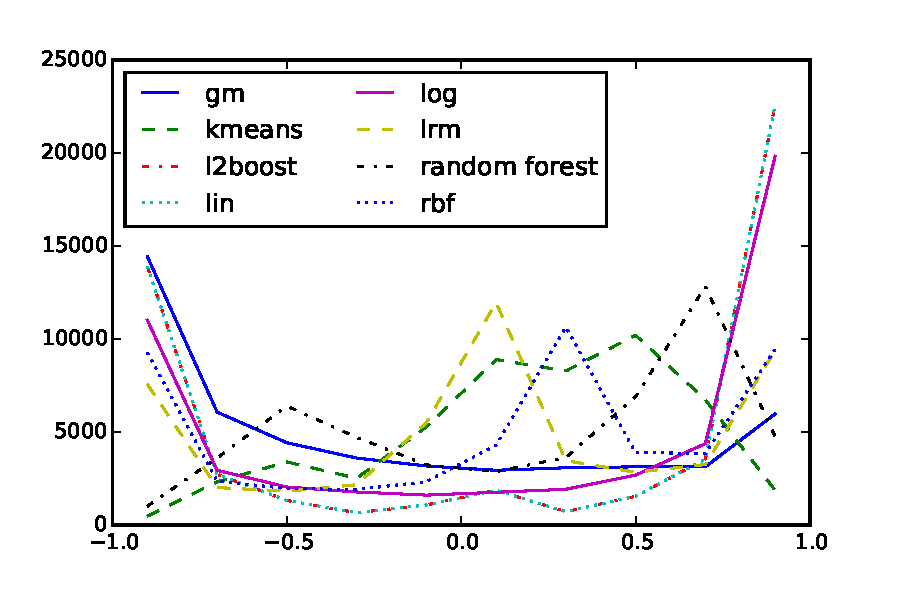
\includegraphics[width=\linewidth]{figures/confidence_dist.pdf}
\caption{Histograms of the training models $f^{(m)}$ (as in \S\ref{sec:ensemble}) on the training set for the single models.  Abbreviations are defined in table~\ref{table:results}.  Some models cluster at \mbox{$+/-1$}.  These may be over-estimating the confidence of predictions. }
\label{fig:confidence_dist}
%\end{figure}
\end{minipage}%
\hfill
\begin{minipage}[t]{0.48\textwidth} 
%\begin{figure}
\centering
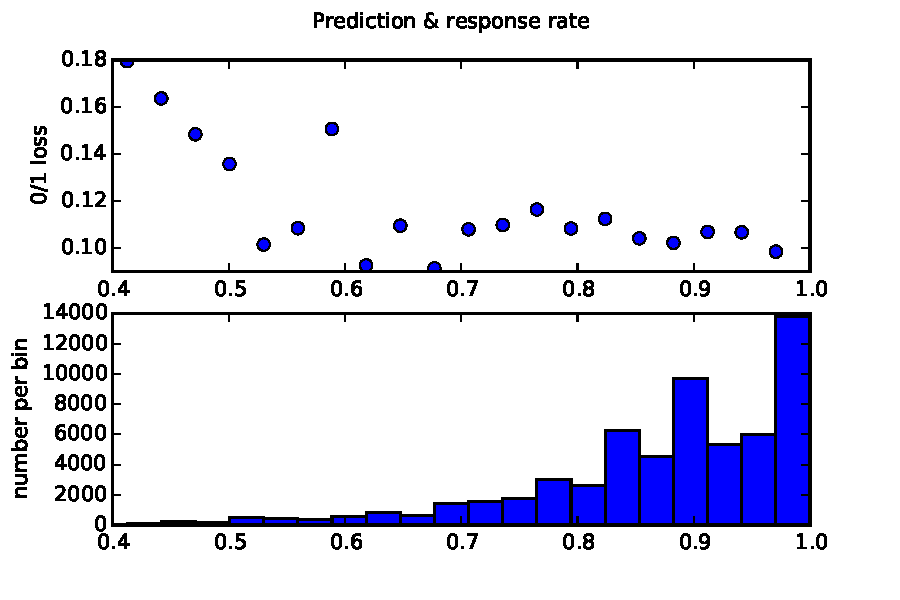
\includegraphics[width=\linewidth]{figures/prediction_response_rate.pdf}
\caption{0/1 loss and response rate for the full feature set.  The x-axis on both panels is the response rate to features (fraction of answered questions averaged over all people). (top panel) 0/1 loss on the training set as a function of individual's response rate.  (bottom panel) Histogram of people's response rates.  0/1 loss decreases with increasing response rate. }
\label{fig:prediction_response_rate}
\end{minipage}
\end{figure}



%
%\subsubsection*{References}
%
%References follow the acknowledgments. Use unnumbered third level heading for
%the references. Any choice of citation style is acceptable as long as you are
%consistent. It is permissible to reduce the font size to `small' (9-point) 
%when listing the references. {\bf Remember that this year you can use
%a ninth page as long as it contains \emph{only} cited references.}
%
%\small{
%[1] Alexander, J.A. \& Mozer, M.C. (1995) Template-based algorithms
%for connectionist rule extraction. In G. Tesauro, D. S. Touretzky
%and T.K. Leen (eds.), {\it Advances in Neural Information Processing
%Systems 7}, pp. 609-616. Cambridge, MA: MIT Press.
%
%[2] Bower, J.M. \& Beeman, D. (1995) {\it The Book of GENESIS: Exploring
%Realistic Neural Models with the GEneral NEural SImulation System.}
%New York: TELOS/Springer-Verlag.
%
%[3] Hasselmo, M.E., Schnell, E. \& Barkai, E. (1995) Dynamics of learning
%and recall at excitatory recurrent synapses and cholinergic modulation
%in rat hippocampal region CA3. {\it Journal of Neuroscience}
%{\bf 15}(7):5249-5262.
%}

\end{document}
